% Тип документа
\documentclass[a4paper,12pt]{extarticle}

% Шрифты, кодировки, символьные таблицы, переносы
\usepackage{cmap}
\usepackage[T2A]{fontenc}
\usepackage[utf8x]{inputenc}
\usepackage[russian]{babel}

% Это пакет -- хитрый пакет, он нужен но не нужен
\usepackage[mode=buildnew]{standalone}

\usepackage
	{
		% Дополнения Американского математического общества (AMS)
		amssymb,
		amsfonts,
		amsmath,
		amsthm,
		% misccorr,
		% 
		% Графики и рисунки
		wrapfig,
		graphicx,
		subcaption,
		float,
		tikz,
		tikz-3dplot,
		caption,
		csvsimple,
		color,
		booktabs,
		pgfplots,
		pgfplotstable,
		geometry,
		% 
		% Таблицы, списки
		makecell,
		multirow,
		indentfirst,
		%
		% Интегралы и прочие обозначения
		ulem,
		esint,
		esdiff,
		% 
		% Колонтитулы
		fancyhdr,
	}  


% Обводка текста в TikZ
\usepackage[outline]{contour}

% Увеличенный межстрочный интервал, французские пробелы
\linespread{1.3} 
\frenchspacing 

 
\usetikzlibrary
	{
		decorations.pathreplacing,
		decorations.pathmorphing,
		patterns,
		calc,
		scopes,
		arrows,
		fadings,
		through,
		shapes.misc,
		arrows.meta,
		3d,
		quotes,
		angles,
		babel
	}


\tikzset{
	force/.style=	{
		>=latex,
		draw=blue,
		fill=blue,
				 	}, 
	%				 	
	axis/.style=	{
		densely dashed,
		blue,
		line width=1pt,
		font=\small,
					},
	%
	th/.style=	{
		line width=1pt},
	%
	acceleration/.style={
		>=open triangle 60,
		draw=magenta,
		fill=magenta,
					},
	%
	inforce/.style=	{
		force,
		double equal sign distance=2pt,
					},
	%
	interface/.style={
		pattern = north east lines, 
		draw    = none, 
		pattern color=gray!60,
					},
	cross/.style=	{
		cross out, 
		draw=black, 
		minimum size=2*(#1-\pgflinewidth), 
		inner sep=0pt, outer sep=0pt,
					},
	%
	cargo/.style=	{
		rectangle, 
		fill=black!70, 
		inner sep=2.5mm,
					},
	%
	caption/.style= {
		midway,
		fill=white!20, 
		opacity=0.9
					},
	%
	}

\newenvironment{tikzpict}
    {
	    \begin{figure}[htbp]
		\centering
		\begin{tikzpicture}
    }
    { 
		\end{tikzpicture}
		% \caption{caption}
		% \label{fig:label}
		\end{figure}
    }


\newcommand{\vbLabel}[3]{\draw ($(#1,#2)+(0,5pt)$) -- ($(#1,#2)-(0,5pt)$) node[below]{#3}}
\newcommand{\vaLabel}[3]{\draw ($(#1,#2)+(0,5pt)$) node[above]{#3} -- ($(#1,#2)-(0,5pt)$) }

\newcommand{\hrLabel}[3]{\draw ($(#1,#2)+(5pt,0)$) -- ($(#1,#2)-(5pt,0)$) node[right, xshift=1em]{#3}}
\newcommand{\hlLabel}[3]{\draw ($(#1,#2)+(5pt,0)$) node[left, xshift=-1em]{#3} -- ($(#1,#2)-(5pt,0)$) }



\newcommand\zi{^{\,*}_i}
\newcommand\sumn{\sum_{i=1}^{N}}

\tikzset{
	coordsys/.style={scale=1.8,x={(1.1cm,-0cm)},y={(0.5cm,1cm)}, z={(0cm,0.8cm)}},
	coordsys/.style={scale=1.5,x={(0cm,0cm)},y={(1cm,0cm)}, z={(0cm,1cm)}}, 
	coordsys/.style={scale=1.5,x={(1cm,0cm)},y={(0cm,1cm)}, z={(0cm,0cm)}}, 
}

\usepgfplotslibrary{units}


% Draw line annotation
% Input:
%   #1 Line offset (optional)
%   #2 Line angle
%   #3 Line length
%   #5 Line label
% Example:
%   \lineann[1]{30}{2}{$L_1$}

\newcommand{\lineann}[4][0.5]{%
    \begin{scope}[rotate=#2, blue,inner sep=2pt, ]
        \draw[dashed, blue!40] (0,0) -- +(0,#1)
            node [coordinate, near end] (a) {};
        \draw[dashed, blue!40] (#3,0) -- +(0,#1)
            node [coordinate, near end] (b) {};
        \draw[|<->|] (a) -- node[fill=white, scale=0.8] {#4} (b);
    \end{scope}
}

\newcommand{\lineannn}[4][0.5]{%
    \begin{scope}[rotate=#2, blue,inner sep=2pt, ]
        \draw[dashed, blue!40] (0,0) -- +(0,#1)
            node [coordinate, near end] (a) {};
        \draw[dashed, blue!40] (#3,0) -- +(0,#1)
            node [coordinate, near end] (b) {};
        % \draw[color=white, color=blue] (a) -- node[fill=white, scale=0.8] {#4} (b);
        \draw[->|] (a)++(-0.3,0) -- (a);
        \draw[->|] (b)++(0.3,0) coordinate (xx) -- (b);
        \draw (xx) node[fill=white, scale=0.8, right] {#4};
    \end{scope}
}

% Круговая стрелка относительно центра (дуга из центра)
\tikzset{
  pics/carc/.style args={#1:#2:#3}{
    code={
      \draw[pic actions] (#1:#3) arc(#1:#2:#3);
    }
  },
  dash/.style={
  	dash pattern=on 5mm off 5mm
  }
}

% Среднее <#1>
\newcommand{\mean}[1]{\langle#1\rangle}

\pgfplotsset{
    % most recent feature set of pgfplots
    compat=newest,
}

% const прямым шрифтом
\newcommand\ct[1]{\text{\rmfamily\upshape #1}}
\newcommand*{\const}{\ct{const}}


\usepackage[europeanresistors,americaninductors]{circuitikz}

% Style to select only points from #1 to #2 (inclusive)
\pgfplotsset{select/.style 2 args={
    x filter/.code={
        \ifnum\coordindex<#1\def\pgfmathresult{}\fi
        \ifnum\coordindex>#2\def\pgfmathresult{}\fi
    }
}}


\usepackage{array}
\usepackage{pstool}


%%%%%%%%%%%%%%%%%%%%%%%%%%%%%%%%%%%%%%%%%%%%%%%%%
\makeatletter
\newif\if@gather@prefix 
\preto\place@tag@gather{% 
  \if@gather@prefix\iftagsleft@ 
    \kern-\gdisplaywidth@ 
    \rlap{\gather@prefix}% 
    \kern\gdisplaywidth@ 
  \fi\fi 
} 
\appto\place@tag@gather{% 
  \if@gather@prefix\iftagsleft@\else 
    \kern-\displaywidth 
    \rlap{\gather@prefix}% 
    \kern\displaywidth 
  \fi\fi 
  \global\@gather@prefixfalse 
} 
\preto\place@tag{% 
  \if@gather@prefix\iftagsleft@ 
    \kern-\gdisplaywidth@ 
    \rlap{\gather@prefix}% 
    \kern\displaywidth@ 
  \fi\fi 
} 
\appto\place@tag{% 
  \if@gather@prefix\iftagsleft@\else 
    \kern-\displaywidth 
    \rlap{\gather@prefix}% 
    \kern\displaywidth 
  \fi\fi 
  \global\@gather@prefixfalse 
} 
\newcommand*{\beforetext}[1]{% 
  \ifmeasuring@\else
  \gdef\gather@prefix{#1}% 
  \global\@gather@prefixtrue 
  \fi
} 
\makeatother
%%%%%%%%%%%%%%%%%%%%%%%%%%%%%%%%%%%%%%%%%%%%%%%%%

\geometry		
	{
		left			=	2cm,
		right 			=	2cm,
		top 			=	3cm,
		bottom 			=	3cm,
		bindingoffset	=	0cm
	}

%%%%%%%%%%%%%%%%%%%%%%%%%%%%%%%%%%%%%%%%%%%%%%%%%%%%%%%%%%%%%%%%%%%%%%%%%%%%%%%



	%применим колонтитул к стилю страницы
\pagestyle{fancy} 
	%очистим "шапку" страницы
\fancyhead{} 
	%слева сверху на четных и справа на нечетных
\fancyhead[R]{\labauthors} 
	%справа сверху на четных и слева на нечетных
\fancyhead[L]{Отчёт по лабораторной работе №\labnumber} 
	%очистим "подвал" страницы
\fancyfoot{} 
	% номер страницы в нижнем колинтуле в центре
\fancyfoot[C]{\thepage} 

%%%%%%%%%%%%%%%%%%%%%%%%%%%%%%%%%%%%%%%%%%%%%%%%%%%%%%%%%%%%%%%%%%%%%%%%%%%%%%%

\renewcommand{\contentsname}{Оглавление}

\usepackage{tocloft}
% \renewcommand{\cftpartleader}{\cftdotfill{\cftdotsep}} % for parts
% \renewcommand{\cftsectiondotsep}{\cftdotsep}% Chapters should use dots in ToC
\renewcommand{\cftsecleader}{\cftdotfill{\cftdotsep}}
%\renewcommand{\cftsecleader}{\cftdotfill{\cftdotsep}} % for sections, if you really want! (It is default in report and book class (So you may not need it).
% ---------
% \newcommand{\cftchapaftersnum}{.}%
% \usepackage{titlesec}
% \titlelabel{\thetitle.\quad}
\usepackage{secdot}
\sectiondot{subsection}
\usepackage{setspace}

\begin{document}

\def\labauthors{Понур К.А., Сарафанов Ф.Г., Сидоров Д.А.}
\def\labgroup{420}
\def\labnumber{999}
\def\labtheme{Изучение интерференции в схеме с бипризмой Френеля}
\renewcommand{\vec}{\mathbf}
\renewcommand{\Re}{\operatorname{Re}}
\renewcommand{\Im}{\operatorname{Im}}
\renewcommand{\phi}{\phi}
\renewcommand{\kappa}{\varkappa}
\renewcommand{\hat}{\widehat}
\renewcommand{\epsilon}{\varepsilon}
\renewcommand{\phi}{\varphi}
%%%%%%%%%%%%%%%%%%%%%%%%%%%%%%%%%%%%%%%%%%%%%%%%%%%%%%%%%%%%%%%%%%%%%%%%%%%%%%%
\begin{titlepage}

\begin{center}

{\small\textsc{Нижегородский государственный университет имени Н.\,И. Лобачевского}}
\vskip 1pt \hrule \vskip 3pt
{\small\textsc{Радиофизический факультет}}

\vfill

{\Large Отчет по лабораторной работе №\labnumber\vskip 12pt\bfseries \labtheme}
	
\end{center}

\vfill
	
\begin{flushright}
	{Выполнили студенты \labgroup\ группы\\ \labauthors}%\vskip 12pt Принял:\\ Менсов С.\,Н.}
\end{flushright}
	
\vfill
	
\begin{center}
	Нижний Новгород, \the\year
\end{center}

\end{titlepage}


%%%%%%%%%%%%%%%%%%%%%%%%%%%%%%%%%%%%%%%%%%%%%%%%%%%%%%%%%%%%%%%%%%%%%%%%%%%%%%%
\begin{spacing}{1}
\tableofcontents
\end{spacing}
% \setstretch{1.2}
\newpage
%%%%%%%%%%%%%%%%%%%%%%%%%%%%%%%%%%%%%%%%%%%%%%%%%%%%%%%%%%%%%%%%%%%%%%%%%%%%%%%


 \section{Изучение интерференции в схеме с бипризмой Френеля}
\subsection{Введение}

Цель работы -- целью данной работы является получение интерфереционной картины, проверка некоторых теоретических формул
и определение средней длины волны света, пропускаемого красным и зеленым светофильтрами.
В данной работе для получения когерентных источников света применяется способ, предложенный Френелем и связанный с использованием бипризмы.
\subsection{Теоретическая часть}
В произвольной точке экрана результирующая интенсивность $I(x)$ есть усредненное за время регистрации $\tau$ значение квадрата напряженности суммарного электрического поля:
\begin{gather}
\label{eq:1}
	\vec{E}(r,t)=\vec{E_1}(r_1,t)+\vec{E_2}(r_2,t)=\\=
	-\vec{A_1}(r_1)\cos(\omega t-kr_1+\phi_1)+\vec{A_2}(r_2)
		\cos(\omega t -kr_2+\phi_2), \text{то есть} \nonumber
\end{gather}
\begin{equation}
	I(x)=A_1^2+A_2^2+2(\vec{A_1},\vec{A_2})\cos[k(r_2-r_1-(\phi_2-\phi_1)]
\end{equation}
Бипризма представляет собой две соединенные своими основаниями призмы с одинаковыми и очень малыми (порядка долей градуса) преломляющими углами. 

Каждая из половинок бипризмы отклоняет падающие на неё лучи к своему основанию и поворачивает тем самым фронт волны.  Продолжения лучей, отклоненных первой половиной бипризмы, пересекаются в точке $S_1$, которую можно рассматривать как мнимый источник света. Продолжения всех лучей, отконенных второй половиной бипризмы, пересекаются в точке $S_2$, которую можно рассматривать как другой мнимый источник света. Так как лучи, отклоненные обеими половинками бипризмы, падают на неё от одногои того же источника света, то мнимые источники света $S_1$ и $S_2$ будут когерентны. 

Та область, в которой распространяет- ся волне, отклоненная одной только первой половиной бипризмы, на рис. 3 заштрихована линиями, параллельными $OA$. Та область, в которой распространяется волна, отклоненная одной только второй половиной бипризмы, заштрихована линиями, параллельными $OB$. В области $OMN$ , покрытой на рис. 3 двойной
штриховкой, происходит наложение двух когерентных волн от двух мнимых источников $S_1$, и $S_2$. В этой области пространства имеют место явления интерференции и на участке $MN$ экрана
наблюдения мы увидим ряд светлых и темных (при освещении белым светом - окрашенных) интерференционных полос.

\begin{figure}[H]
	\centering
	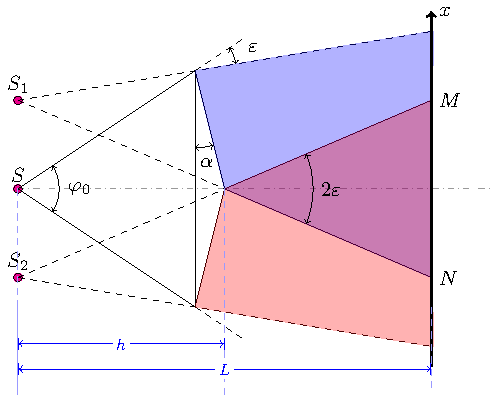
\includegraphics[width=0.55\textwidth]{ris/ris3}
	\caption{ }
	\label{fig:ris3}
\end{figure}
При построении хода лучей, отклоняемых бипризмой (\ref{fig:ris3}) в случае малого преломляющего угла ы. бипризмы и малых углов падения лучей на призму можно воспользоваться следующей приближенной формулой для угла отклонения $\epsilon$
Согласно этому выражению угол отклонении призмой лучей в рассматриваемом приближении не зависит от угля падения и целиком определяется материалом и геометрией призмы. Так, например, если показатель преломления стекла, из которого сделана бипризма, $n=1.5$, то угол отклонения $\epsilon$ просто равен половине преломляющего угла $\alpha$ призмы:
\begin{equation}
 	\epsilon=\frac{\alpha}{2}
 \end{equation} 

Воспользовавшись формулой $s$ или $s$ и выполнив построение хода лучей, можно убедиться в том, что, если $SO\bot AB$ (\ref{fig:ris3}), то мнимые изображения и	действительного источника света $S$ лежат в одной плоскости с действительным источником, причем эта плоскость параллельна передней грани бипризмы. Это обстоятельство в дальнейшем облегчит нам нахождение расстояния $\delta$ между мнимыми источниками $S_1$ и	$S_2$.
Ограничения поля интерференции $MN$ за бипризмой зависят от величины предельного угла расходимости $\phi_0$ светового пучка, падающего на бипризму от щели $S$. Особый интерес представляют два частных случая:

1. При $\phi_0 = 2\epsilon$	линейная ширина поля интерференции,
начиная с расстояния $h$ за бипризмой, остается неизменной и равна расстоянию $\delta$ между мнимыми источниками $S_1$ и $S_2$.

2. При $h\rightarrow\infty$,что можно осуществить,
осветив бипризму параллельным пучком лучей, полученным с помощью вспомогательной линзы (\ref{fig:ris4}), сечение поля интерференции имеет форму ромба. Максимальная ширина поля интерференции $MN$ в этом случае равна половине ширины параллельного пучка падающего на бипризму. Такая схема интерференции соответствует cлучаю наложения двух параллельных когерентных световых пучков
пересекающих друг друга под постоянным углом.
\begin{figure}[H]
	\centering
	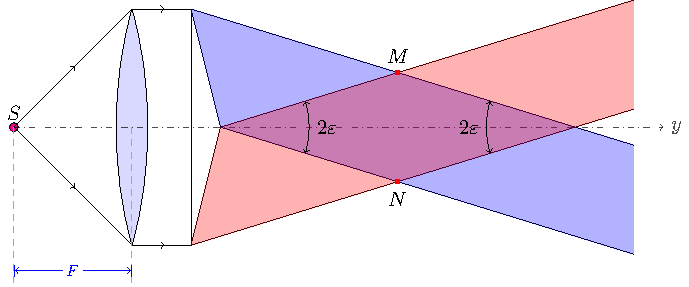
\includegraphics[width=0.85\textwidth]{ris/ris4}
	\caption{ }
	\label{fig:ris4}
\end{figure}
Для расчета наблюдаемой на экране интерференционной картины воспользуемся тем, что бипризма Френеля так изменяет ход лучей от действительного источника, что дает нам право рассматривать световое возмущение в области $MN$ (\ref{fig:ris3}) как результат синфазного излучения двух мнимых источников $S_1$ и $S_2$. При этом рассматривая выражение (\ref{eq:1})для соответствующих проекций $\vec{E_1}(r,t)$ $\vec{E_2}(r,t)$, пренебрежем зависимостью амплитуд $A_1$ и $A_2$ от расстояния $r$, то есть будем считать $A_1=A_2=A_0$	и положим $\phi_1=\phi_2=0$.

Найдем как ширина $d$ полос интерференции зависит от параметров нашей измерительной установки, то есть от длины установки $L$,расстояния между мнимыми источниками и длины волны света  
$\lambda$, испускаемого действиткльным источником $S$. В точку $P$ на экране $MN$ колебания источников $S_1$ и $S_2$ придут с разностью хода:
\begin{equation}
	\Delta=S_2B=r_2-r_1
\end{equation}
и, следовательно, с разностью фаз
\begin{equation}
	\phi(x)=\frac{2\pi}{\lambda}(r_2-r_1)
\end{equation}
На основании вышеизложенного и в соответствии с выражением (\ref{eq:1}) интенсивность результирующего колебания в точке наблюдения $P$ с координатой $x$ определяется формулой
\begin{equation}
	I(x)=2A^2[1+\cos{\phi(x)}]=A^2\cos^2{\frac{\phi}{2}}
\end{equation}
Максимумы освещенности будут получаться в тех местах экрана, для которых разность фаз
\begin{equation}
	\phi(x)=\frac{2\pi}{\lambda}\Delta=2\pi m, \text{где} m=0;\pm 1,\pm 2,\cdots
\end{equation}
То есть для которых разность хода
\begin{equation}
	\Delta=r_2-r_1=m\lambda
\end{equation}

Для нахождения координат максимумов интенсивности вычислим разность хода $\Delta=r_2-r_1$. Несложно получить: 
\begin{gather}
	\label{eq:8}
	r_2-r_1=\frac{4ax}{r_1+r_2} \\ \nonumber
	r_1^2=L^2+(x-a)^2 \\ \nonumber
	r_2^2=L^2+(x+a)^2 \nonumber
\end{gather}


Предполагая величины $\frac{x+a}{L}$ и $\frac{x-a}{L}$ малыми, разложим $r_1$ и $r_2$ в ряд и ограничимся двумя членами в разложении. В результате получим
\begin{equation}
	\label{eq:9}
	r_1+r_2\simeq 2L +\frac{x^2+a^2}{L} 
\end{equation}
Подставляя (\ref{eq:9}) в (\ref{eq:8}) найдём, что 
\begin{equation}
	r_2-r_1\simeq \frac{2ax}{L}\left(1-\frac{x^1+a^2}{2l^2} \right) \label{eq:10}
\end{equation}
При условии 
\begin{equation}
	\frac{\delta x(x^2+a^2)}{2L^3}\ll\frac{\lambda}{2}
\end{equation}
которое позволяет в выражении для разности хода (\ref{eq:10}) отбросить слагаемое, дающее малый по сравнению с $\pi$ вклад в разность фаз интерфеиррующих волн, точное выражение (\ref{eq:8}) может быть заменено на приближенное
\begin{equation}
 	r_1-r_2\simeq\frac{\delta x}{L} \label{eq:12}
 \end{equation} 
 Отметим, что выражение (\ref{eq:12}) сразу следует при условии малости угла 
 $\theta (\sin{\theta}\simeq\theta)$ из приближения приближения парралельных лучей. 
 \begin{equation}
 	\Delta=S_2C=\delta\sin{\theta}\simeq\frac{\delta x}{L}
 \end{equation}
 Следовательно, ширина полос интерференции, равная расстоянию между двумя соседними максимумами освещенности в первои приближении равна:
 \begin{equation}
 	x_{m+1}-x_m=d=\frac{L\lambda}{\delta} \label{eq:14}
 \end{equation}
 Формулу (\ref{eq:14}), переписанную в другом виде
 \begin{equation}
 	\delta d=L\lambda
 \end{equation}
 удобно использовать для проверки теории интерференционных явлений. Если оставлять неизменным расстояние $L$ между щелью $S$ и экраном наблюдения и работать с одной и той же длиной волны $\lambda$ (пользоваться одним и тем же светофильтром), то произведение $\delta d$ должно оставаться (согласно теории) постоянным. Таким образом, для проверки теории нужно, меняя расстояние между мнимыми источниками, независимыми способами измерять расстояния $\delta$ и $d$.Если их произведение будет оставаться постоянным (конечно, при $L= \const$ и $\lambda=\const$ ), то это будет служить доказательством правильности изложенной теории. Расстояние $\delta$ между мнимыми источниками в данной работе можно изменять, изменяя величину $h$ (см. рис. ). То есть помещая бипризму на различным расстояниях от щели.
%%%%%%%%%%%%%%%%%%%%%%%%%%%%%%%%%%%%%%%%%%%%%%%%%%%%%%%%%%%%%%%%%%%%%%%%%%%%%%%
\section{Практическая часть}
\subsection{Задание 1}
Была измерена $d$ и ширина щели при двух значениях $h$, при которой происходило размытие картины.  
\subsection{Задание 2}
\begin{figure}[]
	\centering
	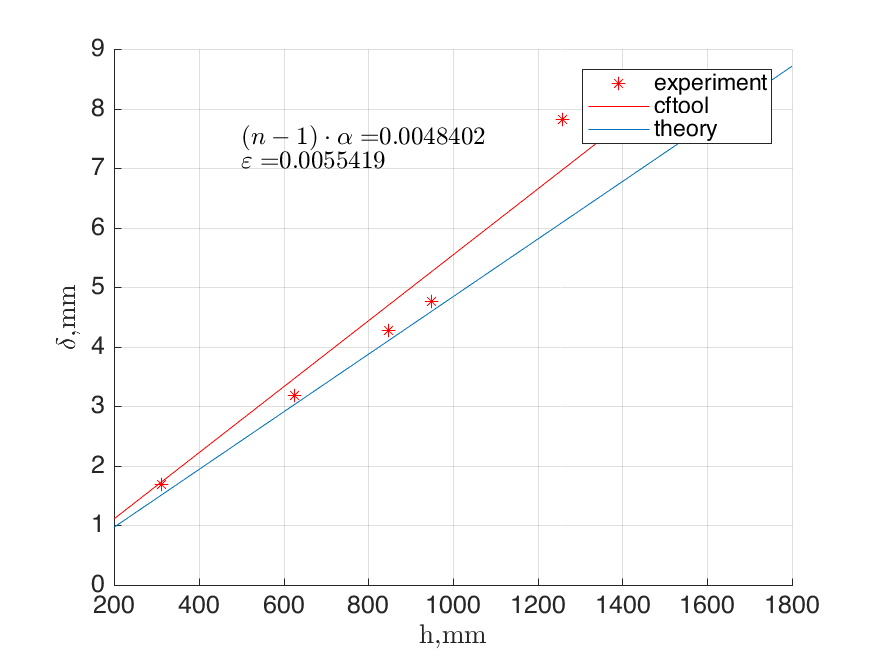
\includegraphics[width=1\textwidth]{data/d_g.png}
	\caption{Зеленый светофильтр}
	\label{fig:d_g}
\end{figure}

\begin{figure}[ht]
\begin{minipage}[b]{0.55\linewidth}

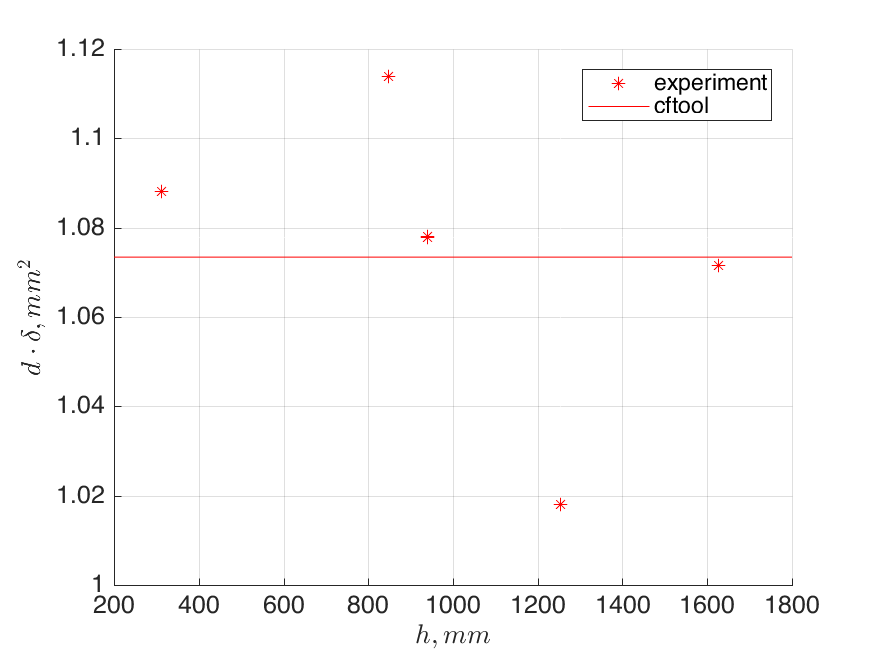
\includegraphics[width=\textwidth]{data/dd_g.png}
\caption{Зеленый светофильтр}
\label{fig:dd_g}
\end{minipage}
\hspace{0.1cm}
\begin{minipage}[b]{0.55\linewidth}
\centering
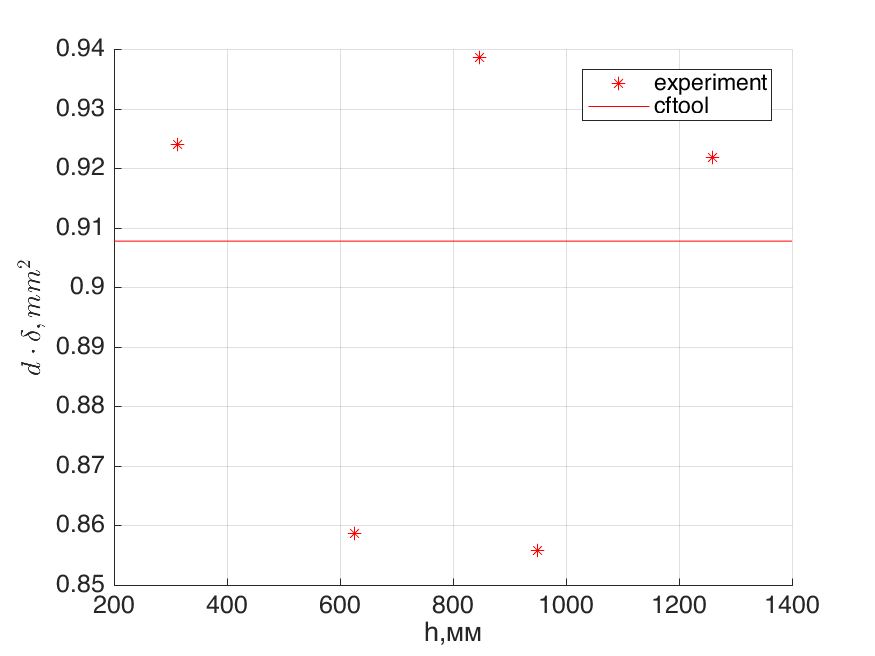
\includegraphics[width=\textwidth]{data/dd_r.png}
\caption{Красный светофильтр}
\label{fig:dd_r}
\end{minipage}
\end{figure}
\begin{figure}[]
	\centering
	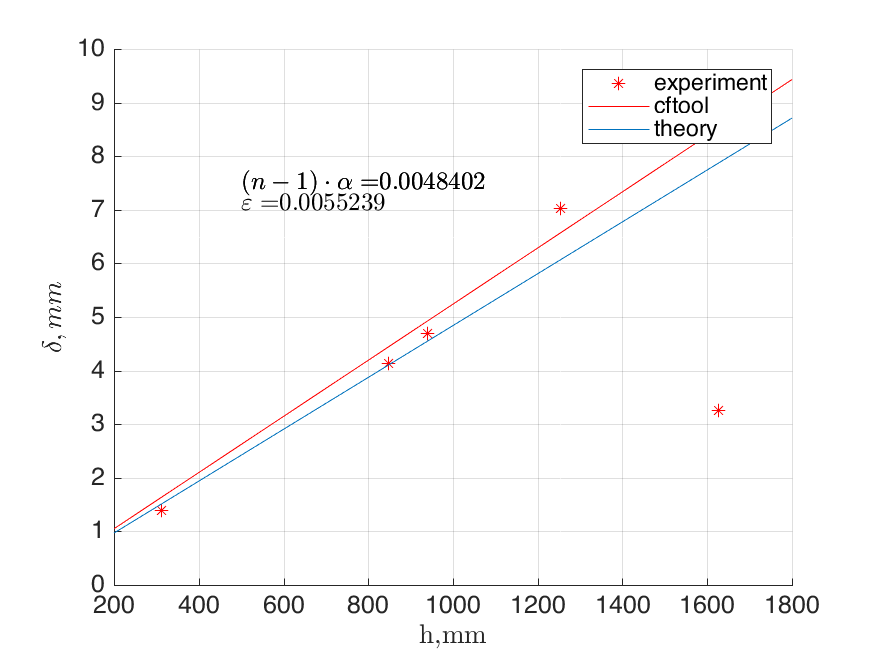
\includegraphics[width=0.\textwidth]{data/d_r.png}
	\caption{Красный светофильтр}
	\label{fig:d_r}
\end{figure}
% \begin{figure}[]
% 	\centering
% 	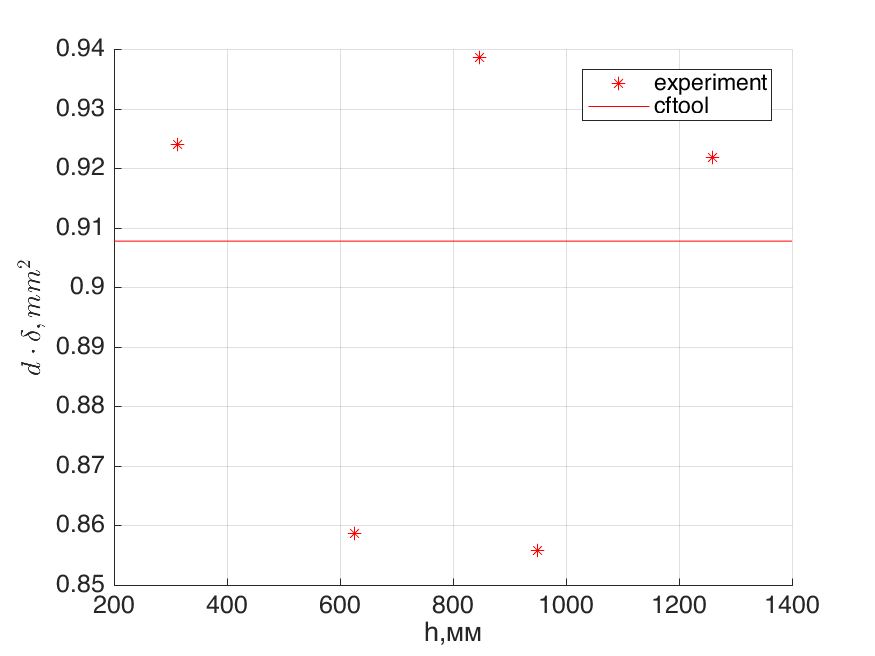
\includegraphics[width=0.\textwidth]{data/dd_r.png}
% 	\caption{}
% 	\label{fig:dd_r}
% \end{figure}
% \begin{figure}[]
% 	\centering
% 	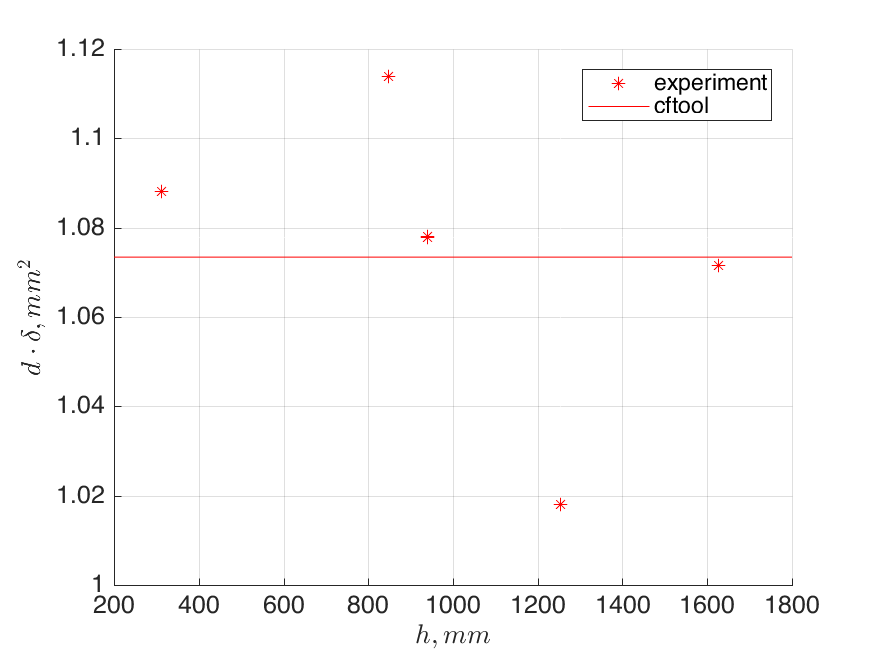
\includegraphics[width=0.\textwidth]{data/dd_g.png}
% 	\caption{}
% 	\label{fig:dr_g}
% \end{figure}
\subsection{Задание 3}
Также из подобия треугольников выводится формула зависимости количества полос $N$ от расстояния $h$ от источника до призмы:
\begin{gather}
	N=\frac{2\delta(L-h)}{dh} \nonumber
\end{gather}
При этом необходимо учесть, что $\delta(h)=2\epsilon h$. Тогда получаем 
\begin{equation}
	N+2\frac{\epsilon^2(Lh-h^2)}{L\lambda}
\end{equation}
Функция принимает максимальное значение при $h=L/2$


\subsection{Задание 4}


\section{Заключение}

\end{document} 